\documentclass[12pt]{article}

\usepackage{sbc-template}
\usepackage{graphicx,url}
\usepackage[utf8]{inputenc}
\usepackage[T1]{fontenc}
\usepackage[brazilian]{babel}
\usepackage{array}

\sloppy

\title{Avaliação da Qualidade do Planejamento de Formatura do No Fluxo UnB:
Requisitos e Especificação segundo a ISO/IEC 25040}

\author{Ana Beatriz Souza Araujo\inst{1}, Giovani De Oliveira Teodoro Coelho\inst{1},\\
  Yasmim de Souza Santos\inst{1}, Gabriel Mota Oliveira\inst{1},\\
  Gustavo Gomes Fornaciari\inst{1}, Vitor Lages Nogueira Araújo\inst{1}}

\address{Faculdade de Ciências e Tecnologias em Engenharia (FCTE)\\
  Universidade de Brasília (UnB) -- Brasília, DF -- Brasil}

\begin{document}

\maketitle

\begin{abstract}
Students at the University of Brasília (UnB) use web tools to understand their
curriculum and plan the courses they still need to take. This paper reports the
first stage of a quality evaluation of the graduation planning flow of No Fluxo
UnB, which receives the student's academic transcript, renders the current
curriculum flowchart and generates a semester-by-semester plan until graduation.
The evaluation follows the ISO/IEC 25040 evaluation process of the SQuaRE family,
uses the Goal-Question-Metric (GQM) method to specify the measures and applies
PSM/CID measures to manage the project. This version covers Phases 1 and 2: the
evaluation requirements, a quality model adapted from ISO/IEC 25010 focused on
Functional Suitability, Security and Usability, and the specification of two
measurement goals, nine questions and twelve metrics with judgment criteria.
\end{abstract}

\begin{resumo}
Estudantes da Universidade de Brasília (UnB) usam ferramentas web para entender a
matriz curricular e planejar as disciplinas que ainda precisam cursar. Este artigo
relata a primeira etapa da avaliação da qualidade do fluxo de planejamento de
formatura do No Fluxo UnB, que recebe o histórico acadêmico do estudante,
apresenta o fluxograma atual do curso e gera um plano de disciplinas por semestre
até a formatura. A avaliação segue o processo da ISO/IEC 25040, da família SQuaRE,
usa o método Goal-Question-Metric (GQM) para especificar as medidas e aplica
medidas do PSM/CID na gestão do projeto. Esta versão cobre as Fases 1 e 2: os
requisitos da avaliação, um modelo de qualidade adaptado da ISO/IEC 25010 com foco
em Adequação Funcional, Segurança e Usabilidade, e a especificação de dois
objetivos de medição, nove questões e doze métricas com critérios de julgamento.
\end{resumo}

\section{Introdução}\label{sec:introducao}

O No Fluxo UnB é uma aplicação web que apresenta a matriz curricular em um
fluxograma interativo e apoia o estudante da Universidade de Brasília (UnB) na
visualização das disciplinas cursadas e no planejamento até a formatura
\cite{nofluxo2026site,nofluxo2026repo}. A ferramenta auxilia o estudante a decidir
quais disciplinas cursar nos próximos semestres e quando poderá concluir o curso.
Um plano com pré-requisitos ignorados, co-requisitos omitidos, disciplinas
obrigatórias ausentes ou histórico interpretado incorretamente pode levar a
decisões acadêmicas inadequadas e até atrasar a graduação. Além disso, o histórico
acadêmico enviado pode conter informações pessoais.

Este trabalho avalia o fluxo de planejamento de formatura da aplicação, composto pelo envio do
histórico acadêmico, pela renderização inicial do fluxograma atual e pela tela
``Planejar formatura'', que gera uma sequência de disciplinas por semestre e uma
previsão de formatura. Essa tela é o objeto central da avaliação.

O objetivo geral é avaliar a qualidade desse fluxo segundo as características
Adequação Funcional, Segurança e Usabilidade do modelo de qualidade da ISO/IEC
25010 \cite{iso25010}. Os objetivos específicos são: (i) estabelecer os requisitos
da avaliação, isto é, propósito, partes interessadas, modelo de qualidade e escopo;
(ii) especificar a avaliação com objetivos, questões, hipóteses, métricas e
critérios de julgamento; (iii) projetar e executar a avaliação; e (iv) propor e
executar ao menos uma ação de melhoria com base nos resultados. Esta primeira versão
do artigo cobre os objetivos (i) e (ii), que correspondem às Fases 1 e 2 do processo
de avaliação.

A abordagem segue o processo de avaliação da família SQuaRE, descrito na ISO/IEC
25040 \cite{iso25040}, usa o método Goal-Question-Metric (GQM)
\cite{basili1994gqm} para derivar as métricas e aplica medidas do PSM/CID
\cite{mcgarry2001psm,psm2021cid} para acompanhar a execução do projeto. Ao final,
a equipe entregará recomendações e ao menos uma ação de melhoria. Os documentos, os
dados e os procedimentos estão no
repositório da
equipe\footnote{\url{https://github.com/FCTE-Qualidade-de-Software-1/2026-2_T02_JEAN_SAMMET}}
e na sua página de
documentação\footnote{\url{https://fcte-qualidade-de-software-1.github.io/2026-2_T02_JEAN_SAMMET/}}.

O restante do artigo está organizado da seguinte forma: a
Seção~\ref{sec:referencial} apresenta o referencial teórico; a
Seção~\ref{sec:metodologia}, a metodologia de desenvolvimento do projeto; as
Seções~\ref{sec:fase1} e~\ref{sec:fase2} descrevem as Fases 1 e 2; e a
Seção~\ref{sec:conclusao} traz as considerações parciais.

\section{Referencial Teórico}\label{sec:referencial}

Esta seção apresenta os conceitos que fundamentam a avaliação: a família de normas
SQuaRE, o modelo de qualidade e o processo de avaliação que ela define, o método
GQM e o PSM/CID.

\subsection{Qualidade de produto de software e a família SQuaRE}\label{sec:square}

A família ISO/IEC 25000, conhecida como SQuaRE (\textit{Systems and software
Quality Requirements and Evaluation}), reúne normas para especificar e avaliar a
qualidade de sistemas e produtos de software e substitui as séries ISO/IEC 9126 e
ISO/IEC 14598 \cite{iso25000}. Ela é organizada em cinco divisões principais: gestão
da qualidade (2500n), modelo de qualidade (2501n), medição da qualidade (2502n),
requisitos de qualidade (2503n) e avaliação da qualidade (2504n), além de uma
divisão de extensão. Neste trabalho são usadas a ISO/IEC 25010, que define o modelo
de qualidade; a ISO/IEC 25020 e a ISO/IEC 25023, que tratam da estrutura de medição e
das medidas de qualidade de produto \cite{iso25020,iso25023}; a ISO/IEC 25030,
sobre requisitos de qualidade \cite{iso25030}; e a ISO/IEC 25040, que descreve o
processo de avaliação.

\subsection{Modelo de qualidade da ISO/IEC 25010}\label{sec:iso25010}

O modelo de qualidade de produto da ISO/IEC 25010:2011 organiza a qualidade em oito
características: adequação funcional, eficiência de desempenho, compatibilidade,
usabilidade, confiabilidade, segurança, manutenibilidade e portabilidade, cada uma
dividida em subcaracterísticas \cite{iso25010}. Três delas são relevantes para este
trabalho. A Adequação Funcional é o grau em que o produto fornece funções que
atendem às necessidades declaradas e implícitas quando usado nas condições
especificadas, e se divide em completude, correção e aptidão funcional. A Segurança
é o grau em que o produto protege informações e dados, de modo que pessoas e
sistemas tenham acesso apenas no nível adequado à sua autorização; suas
subcaracterísticas são confidencialidade, integridade, não repúdio,
responsabilização e autenticidade. A Usabilidade é o grau em que o produto pode ser
usado por usuários específicos para atingir objetivos com eficácia, eficiência e
satisfação em um contexto de uso, e inclui, entre outras, apreensibilidade e
operabilidade. A edição de 2023 da norma revisou o modelo e renomeou algumas
características \cite{iso25010v2023}; este trabalho adota a edição de 2011.

\subsection{Processo de avaliação da ISO/IEC 25040}\label{sec:iso25040}

A ISO/IEC 25040 define o processo de avaliação da qualidade de produto em cinco
atividades: estabelecer os requisitos da avaliação, especificar, projetar, executar
e concluir a avaliação \cite{iso25040}. Na primeira, definem-se o propósito, os
requisitos de qualidade, as partes do produto incluídas e o rigor da avaliação. Na
segunda, selecionam-se as medidas de qualidade e definem-se os critérios de decisão
para as medidas e para a avaliação. A terceira produz o plano de avaliação; a quarta
realiza as medições e aplica os critérios de decisão; e a quinta revisa os
resultados, produz o relatório e trata os dados da avaliação. A especificação deve
ser detalhada o bastante para que a avaliação seja repetível e reprodutível. Na
disciplina em que este trabalho foi desenvolvido, a conclusão é agrupada com a
execução, o que resulta em quatro fases.

\subsection{Método GQM}\label{sec:gqm}

O GQM é uma abordagem orientada a objetivos para definir medições: em vez de partir
das medidas disponíveis, parte-se do que se deseja saber \cite{basili1994gqm}. O
modelo tem três níveis. No nível conceitual, o objetivo de medição é descrito por um
modelo estruturado que informa o objeto analisado, o propósito, o foco de qualidade,
o ponto de vista e o contexto. No nível operacional, o objetivo é refinado em
questões que caracterizam o objeto em relação ao foco, cada uma acompanhada de uma
hipótese, isto é, a resposta esperada que orienta a interpretação dos resultados.
No nível quantitativo, associam-se a cada questão métricas que permitem respondê-la
de forma objetiva \cite{solingen1999gqm}. As métricas devem ser simples, objetivas,
fáceis de coletar e válidas, ou seja, devem medir o que se pretende medir.

\subsection{Medição para gestão de projetos: PSM/CID}\label{sec:psm}

O PSM (\textit{Practical Software and Systems Measurement}) é uma abordagem de
medição dirigida por necessidades de informação e ligada à gestão de projetos
\cite{mcgarry2001psm}. Seu modelo de informação, alinhado à ISO/IEC/IEEE 15939
\cite{iso15939}, liga uma necessidade de informação a um conceito mensurável e às
entidades e atributos medidos. Medidas básicas são obtidas por um método de
medição, combinadas em medidas derivadas por uma função de medição e transformadas
em indicadores por um modelo de análise com critérios de decisão. O PSM organiza as
necessidades de informação em categorias como calendário e progresso, recursos e
custos, tamanho e estabilidade, qualidade do produto e desempenho do processo. O
\textit{framework} PSM/CID adapta essa abordagem ao desenvolvimento contínuo e
iterativo, com uma tabela de categorias, conceitos mensuráveis e medidas e com
especificações de medidas como \textit{burndown}, comprometido versus concluído,
tempo de ciclo e velocidade da equipe \cite{psm2021cid}.

\section{Metodologia de Desenvolvimento do Projeto}\label{sec:metodologia}

A equipe adotou uma metodologia composta e adaptada para este projeto, orientada
pela família SQuaRE. Ela combina três abordagens estabelecidas, cada uma com um
papel definido: o processo da ISO/IEC 25040 conduz a avaliação do produto, o GQM
especifica as métricas da Fase 2 e o PSM/CID mede a gestão do próprio projeto. As
duas frentes de medição usam o modelo de informação da ISO/IEC/IEEE 15939, no qual
também se apoia a estrutura de medição da ISO/IEC 25020, o que permite tratar com os
mesmos conceitos de necessidade de informação, medida e critério de decisão a
avaliação do produto e a gestão da equipe. A forma de integrar as abordagens e o
fluxo de trabalho descrito a seguir são adaptações da equipe, e não partes das
referências citadas.

\subsection{Processo adotado}\label{sec:processo}

As quatro fases do processo de avaliação foram distribuídas entre as entregas da
disciplina: a Entrega 1, em 26/10/2026, cobre as Fases 1 e 2, e a Entrega 2 cobre as
Fases 3 e 4, incluindo a ação de melhoria. Cada entrega é tratada como um ciclo
iterativo, que começa com o planejamento das tarefas, segue com a execução e a
revisão por outro integrante, termina com a integração ao repositório e é
acompanhado pelas medições do PSM/CID, cujos resultados orientam o ajuste do ciclo
seguinte. A documentação detalhada de cada fase é publicada na página de
documentação do projeto, e este artigo é a síntese dessa documentação.

\subsection{Organização da equipe, ferramentas e artefatos}\label{sec:organizacao}

A equipe é formada por seis integrantes. Em cada entrega, o trabalho é dividido em
frentes registradas como \textit{Issues} no GitHub e associadas a um
\textit{Milestone}. Na Entrega 1, as frentes foram introdução e referencial teórico,
objetivos, questões e métricas GQM, gráfico GQM, gestão com PSM/CID, estruturação
da página de documentação e compilação da versão em LaTeX, cada uma sob
responsabilidade de uma dupla. Cada tarefa é desenvolvida em uma \textit{branch}
própria e integrada à \textit{branch} principal por \textit{Pull Request}, e a
revisão por um integrante diferente do autor faz parte do critério de conclusão. A
página de documentação é construída com MkDocs Material e publicada automaticamente
a cada atualização da \textit{branch} principal; os diagramas são versionados em
Mermaid, e o artigo é escrito em LaTeX com o modelo da SBC. Uma tarefa só é
concluída quando atende aos critérios de avaliação da disciplina, como a ligação
explícita com a fase anterior, o uso da terminologia da ISO/IEC 25010, figuras e
tabelas com legenda e fonte e a declaração do uso de IA.

\subsection{Gestão do projeto com PSM/CID}\label{sec:gestao}

A gestão do projeto usa as três categorias de informação exigidas pela disciplina,
com dados extraídos do repositório Git. Para cada categoria, a equipe definiu uma
necessidade de informação, as medidas e os critérios de decisão
(Tabela~\ref{tab:psm}).

\begin{table}[!ht]
\centering
\caption{Medidas PSM/CID usadas na gestão do projeto. Fonte: elaboração da equipe.}
\label{tab:psm}
\footnotesize
\begin{tabular}{|>{\raggedright\arraybackslash}p{2.2cm}|>{\raggedright\arraybackslash}p{3.0cm}|>{\raggedright\arraybackslash}p{3.6cm}|>{\raggedright\arraybackslash}p{4.4cm}|}
\hline
\textbf{Categoria} & \textbf{Necessidade de informação} & \textbf{Medida derivada} & \textbf{Critério de decisão} \\ \hline
Calendário e Progresso & A equipe cumpre o cronograma do \textit{Milestone}? & $TCT = N_{conc} / N_{plan} \times 100$ & Meta de 100\% no prazo; se $TCT < 75\%$ a 24 horas do prazo, redistribuir as pendências prioritárias. \\ \hline
Recursos e Custos & A distribuição das tarefas está equilibrada? & $DTI_i = N_i / N_{total} \times 100$; $MTI = N_{total} / N_{integrantes}$ & Revisar a distribuição se um integrante concentrar mais de 35\% das \textit{Issues} ativas ou se afastar mais de 20\% da média. \\ \hline
Desempenho do Processo & As tarefas são concluídas no tempo esperado? & Tempo de ciclo $TC = T_{\mbox{\scriptsize conclusão}} - T_{\mbox{\scriptsize criação}}$; tempo sem atividade $TSA$ & Meta de $TC$ médio de até 2 dias; verificar \textit{Issues} sem atividade há mais de 3 dias. \\ \hline
\end{tabular}
\end{table}

Na Entrega 1, o \textit{Milestone} 1 teve seis \textit{Issues} planejadas, e as
seis foram concluídas até o prazo do marco, em 18/10/2026, o que resulta em
$TCT = 100\%$.

\subsection{Rastreabilidade dos dados e aspectos éticos}\label{sec:rastreabilidade}

Os dados de coleta e de consolidação, os procedimentos de cálculo e as atas das
reuniões são versionados no repositório, de modo que cada número apresentado possa
ser conferido, e cada arquivo de dados identifica a métrica, a data, o ambiente e a
versão do software avaliado. Os testes funcionais usam históricos sintéticos ou
autorizados, sem dados de terceiros. Os testes de usabilidade e eventuais
entrevistas só são gravados com o consentimento dos participantes, que são
identificados por códigos, e as condições de acesso às gravações são definidas
antes da coleta. As verificações de segurança são não invasivas: não há tentativas
de explorar vulnerabilidades ou de contornar a autenticação no sistema em produção.

\section{Fase 1: Estabelecimento dos Requisitos da Avaliação}\label{sec:fase1}

A Fase 1 define os requisitos que precisam estar estabelecidos antes da escolha das
métricas: o propósito da avaliação, as partes interessadas, a descrição do produto,
o modelo de qualidade, as características priorizadas e o escopo.

\subsection{Propósito da avaliação e uso pretendido}\label{sec:proposito}

O No Fluxo UnB auxilia estudantes a consultar a estrutura curricular e a organizar
disciplinas futuras, e informações incompletas ou incorretas podem confundir o
estudante e influenciar seu planejamento. A avaliação tem o propósito de produzir
evidências sobre a adequação funcional, a segurança observável e a usabilidade do
fluxo de planejamento de formatura, para apoiar três decisões: identificar
divergências funcionais que merecem correção ou investigação, a partir de casos de
teste com resultados esperados e observados; identificar problemas observáveis de
acesso ou de exposição de dados, a partir de verificações não invasivas; e
identificar dificuldades no uso do fluxo, a partir do sucesso nas tarefas, dos erros
e dos pedidos de ajuda. Os resultados serão usados pela equipe avaliadora e, se
compartilhados, pelos mantenedores. A avaliação não certifica o software nem substitui a conferência das
regras acadêmicas com as fontes oficiais da UnB.

\subsection{Requisitante e partes interessadas}\label{sec:stakeholders}

A requisitante da avaliação é a professora da disciplina de Qualidade de Software 1.
A Tabela~\ref{tab:stakeholders} resume as partes interessadas, suas necessidades e a
forma como influenciam a avaliação.

\begin{table}[!ht]
\centering
\caption{Partes interessadas na avaliação. Fonte: elaboração da equipe.}
\label{tab:stakeholders}
\footnotesize
\begin{tabular}{|>{\raggedright\arraybackslash}p{2.6cm}|>{\raggedright\arraybackslash}p{2.3cm}|>{\raggedright\arraybackslash}p{4.0cm}|>{\raggedright\arraybackslash}p{4.3cm}|}
\hline
\textbf{Parte interessada} & \textbf{Papel} & \textbf{Necessidades} & \textbf{Influência na avaliação} \\ \hline
Estudantes da UnB & Usuários finais & Informações compreensíveis, funções adequadas e tratamento responsável dos dados & Orientam os casos funcionais e as tarefas de usabilidade \\ \hline
Mantenedores do No Fluxo UnB & Responsáveis técnicos pelo produto & Evidências claras e recomendações acionáveis & Delimitam o que pode ser inspecionado no código público; não se presume participação direta \\ \hline
Profa. Cristiane Ramos & Requisitante e avaliadora acadêmica & Processo documentado, justificativas e rastreabilidade & Define os critérios acadêmicos a cumprir \\ \hline
Equipe avaliadora & Planeja e executa a avaliação & Procedimentos viáveis, dados rastreáveis e conclusões justificadas & Define amostra, método e limites de execução \\ \hline
\end{tabular}
\end{table}

Foram considerados três perfis de estudante como cenários de avaliação: quem está
conhecendo a matriz curricular e precisa localizar as disciplinas relevantes; quem
já cursou parte da matriz e precisa distinguir o que foi concluído do que falta
planejar; e quem tem disciplinas pendentes ou equivalências e precisa interpretar o
plano sem supor que o sistema substitui a confirmação oficial.

\subsection{Tipo de produto e descrição do software}\label{sec:produto}

O No Fluxo UnB é uma aplicação web de apoio ao planejamento acadêmico, acessada pelo
navegador. O estudante seleciona o curso, informa o histórico acadêmico por PDF ou
manualmente, visualiza o fluxograma com a situação das disciplinas e pode solicitar
um plano de formatura (Figura~\ref{fig:planejar}). O repositório público
\cite{nofluxo2026repo}, analisado no \textit{commit} 87b5475, organiza o produto em
um \textit{frontend} web, um \textit{backend} em TypeScript/Node.js, migrações e
serviços de dados e autenticação do Supabase, componentes auxiliares de agente e IA
e \textit{scripts} de dados curriculares. Na tela avaliada, o plano é gerado por um
serviço do \textit{backend}, chamado de Motor 2, acionado pela rota
\texttt{POST /planejamento/gerar-plano}.

\begin{figure}[!ht]
\centering
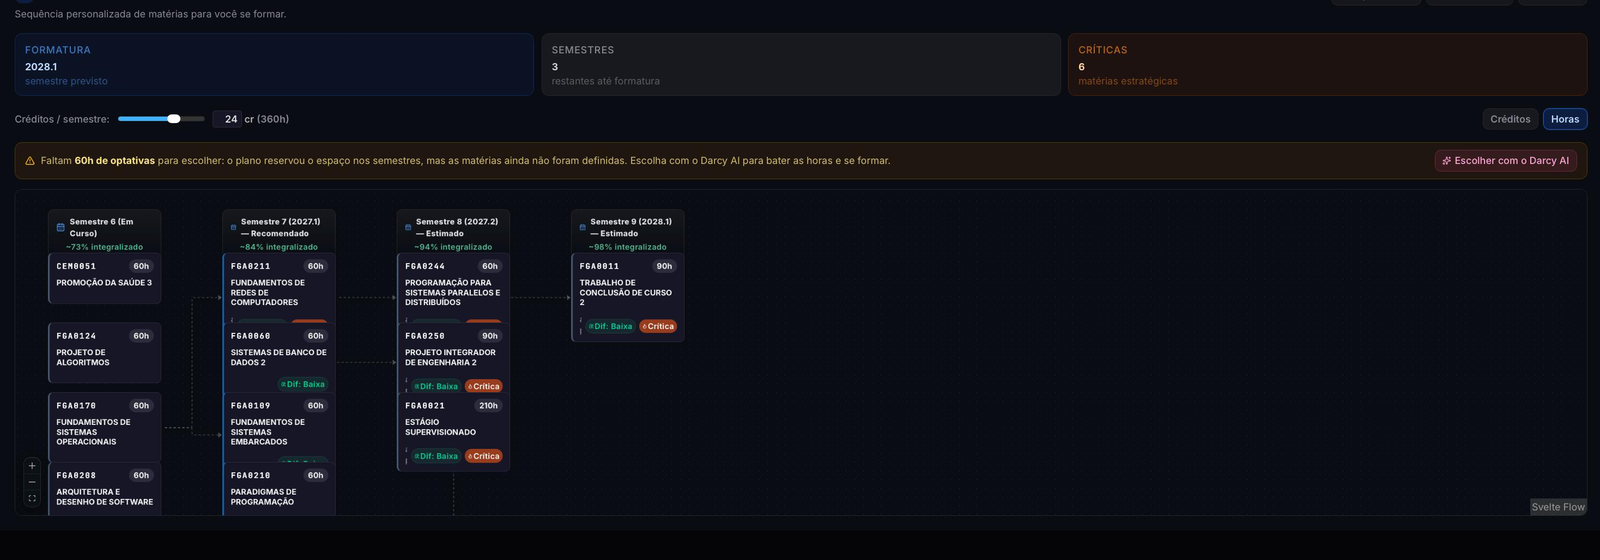
\includegraphics[width=0.95\linewidth]{figuras/noFluxo_planejarFormatura.png}
\caption{Tela ``Planejar formatura'' do No Fluxo UnB, com previsão de formatura,
semestres restantes, matérias críticas e grafo de disciplinas. Fonte: captura de
tela do No Fluxo UnB, outubro de 2026.}
\label{fig:planejar}
\end{figure}

Essa organização tem implicações diretas para a avaliação. Pela interface, é
possível comparar planos gerados para cenários controlados com resultados
esperados, observar participantes executando tarefas e inspecionar, de forma não
invasiva, o armazenamento do navegador e as respostas dos serviços. Não é possível,
com esse recorte, concluir que todos os planos, cursos e históricos estão corretos,
que os resultados representam todos os estudantes da UnB ou que o sistema está livre
de vulnerabilidades. A versão em produção também pode divergir do código público;
por isso, a equipe registra a data, o ambiente e o \textit{commit} analisados.

\subsection{Modelo de qualidade adaptado}\label{sec:modelo}
[PREENCHER]

\subsection{Seleção e priorização das características}\label{sec:priorizacao}
[PREENCHER]

\subsection{Escopo, profundidade e objetos de avaliação}\label{sec:escopo}
[PREENCHER]

\subsection{Relação com os ODS}\label{sec:ods}
[PREENCHER]

\section{Fase 2: Especificação da Avaliação}\label{sec:fase2}
[PREENCHER]

\subsection{Rastreabilidade entre as Fases 1 e 2}\label{sec:rastreabilidade12}
[PREENCHER]

\subsection{Objetivos de medição: nível conceitual}\label{sec:objetivos}
[PREENCHER]

\subsection{Questões e hipóteses: nível operacional}\label{sec:questoes}
[PREENCHER]

\subsection{Métricas: nível quantitativo}\label{sec:metricas}
[PREENCHER]

\subsection{Níveis de pontuação e critérios de julgamento}\label{sec:julgamento}
[PREENCHER]

\subsection{Gráfico GQM}\label{sec:graficogqm}
[PREENCHER]

\section{Considerações Parciais}\label{sec:conclusao}
[PREENCHER]

\section*{Declaração de Uso de Inteligência Artificial}

A equipe usou ferramentas de IA generativa em tarefas de apoio. Ana Beatriz Souza Araujo usou o
Gemini (Google) para organizar os modelos de informação do PSM/CID, formatar tabelas
e revisar a ortografia, e conferiu as fórmulas, os critérios de decisão e os
conceitos com base na literatura do PSM. Gabriel Mota Oliveira usou o ChatGPT para
esboçar textos, revisar a gramática e montar o código Mermaid do GQM, e removeu
trechos sem embasamento ou fora do contexto da disciplina. Giovani De Oliveira
Teodoro Coelho usou o ChatGPT e o Gemini para estruturar hipóteses e métricas
operacionais, diagramar em Mermaid, apoiar a redação dos protocolos de teste e
revisar a ortografia, e ajustou prioridades, fórmulas e procedimentos à Fase 1, às
normas ISO/IEC 25023 e ISO 9241-11 e à LGPD. Gustavo Gomes Fornaciari usou o Claude
(Anthropic) para organizar o repositório e melhorar textos da Fase 1, e desfez
pastas criadas sem necessidade e ajustou o conteúdo ao que havia planejado. Yasmim
de Souza Santos usou o Claude para ajudar a traduzir o modelo do artigo para
LaTeX, validar a documentação feita sobre metodologia e pedir algumas trilhas a serem seguidas para essa pesquisa.

\section*{Disponibilidade dos Dados}

Os documentos, os dados e os procedimentos de cálculo deste trabalho estão
disponíveis no repositório da
equipe\footnote{\url{https://github.com/FCTE-Qualidade-de-Software-1/2026-2_T02_JEAN_SAMMET}}.

\bibliographystyle{sbc}
\bibliography{referencias}

\clearpage
\appendix

\section{Tabela de Contribuição}\label{ap:contribuicao}

\begin{table}[!ht]
\centering
\caption{Contribuição dos integrantes da equipe na Entrega 1. Fonte: elaboração da
equipe.}
\label{tab:contribuicao}
\footnotesize
\begin{tabular}{|>{\raggedright\arraybackslash}p{3.6cm}|p{1.6cm}|>{\raggedright\arraybackslash}p{6.2cm}|>{\centering\arraybackslash}p{1.4cm}|}
\hline
\textbf{Integrante} & \textbf{Matrícula} & \textbf{Atividades realizadas} & \textbf{Esforço (\%)} \\ \hline
Ana Beatriz Souza Araujo & 241025891 & Acompanhamento da gestão do projeto e documentação dessas informações. Também organizou a seção de gestão do projeto, incluindo métricas PSM/CID, acompanhamento de \textit{Issues} e atualização do histórico de versionamento. & 16,66 \\ \hline
Giovani De Oliveira Teodoro Coelho & 241032500 & Elaboração e refinamento das métricas operacionais, com ajustes relacionados à usabilidade, segurança e adequação funcional. Também modularizou a documentação da Fase 2, padronizou referências bibliográficas e contribuiu para o registro do uso de IA. & 16,66 \\ \hline
Yasmim de Souza Santos & 241040860 & Criação do \textit{template} do artigo científico e definição de uma estrutura inicial para sua elaboração. Também reuniu referências bibliográficas de base para orientar a produção do artigo do projeto. & 16,66 \\ \hline
Gabriel Mota Oliveira & 241011081 & Elaboração inicial das perguntas GQM, das fichas de métricas funcionais e do protocolo de cenários de teste. Também estruturou e dividiu páginas da documentação, adicionou referências para as métricas funcionais e contribuiu para a documentação das métricas operacionais e dos critérios de avaliação da Fase 2. & 16,66 \\ \hline
Gustavo Gomes Fornaciari & 241032519 & Organização e estruturação inicial do repositório, configuração do MkDocs e divisão da documentação em páginas. Responsável pela conclusão da Fase 1, incluindo a documentação do software escolhido, propósito e \textit{stakeholders}, escopo, modelo e características de qualidade, além da página de ODS e da manutenção dos critérios e históricos de versionamento. & 16,66 \\ \hline
Vitor Lages Nogueira Araújo & 242025054 & Criação e organização de \textit{Issues} e \textit{Milestones} para acompanhar as atividades e o progresso do projeto. Também realizou atualizações no README, contribuindo para a identificação dos integrantes e a apresentação inicial do repositório. & 16,66 \\ \hline
\end{tabular}
\end{table}

\end{document}
